
% =========================================================
% LinkedIn Carousel (Portrait 4:5) — Fama-French Factor Model
% Real data from Kenneth French's Data Library
% =========================================================

\documentclass{beamer}

% ----------------------------
% Page: portrait 4:5
% ----------------------------
\setlength{\paperwidth}{14.4cm}
\setlength{\paperheight}{18.0cm}
\setlength{\pdfpagewidth}{\paperwidth}
\setlength{\pdfpageheight}{\paperheight}

% ----------------------------
% Packages
% ----------------------------
\usepackage[T1]{fontenc}
\usepackage{amsmath,amssymb}
\usepackage{booktabs}
\usepackage{graphicx}
\usepackage{tikz}
\usetikzlibrary{arrows.meta,positioning,shapes.geometric,calc,
  decorations.pathreplacing,backgrounds}
\usepackage{pgfplots}
\pgfplotsset{compat=1.18}

\usepackage{bookmark}
\usepackage{hyperref}
\hypersetup{
  pdftitle    = {Fama-French Factor Model},
  pdfauthor   = {Muiz Olasupo},
  pdfsubject  = {Quantitative Finance},
  colorlinks  = false,
}

% ----------------------------
% Colors
% ----------------------------
\definecolor{ink}{RGB}{12,14,18}
\definecolor{muted}{RGB}{100,106,115}
\definecolor{soft}{RGB}{245,247,250}
\definecolor{linegray}{RGB}{210,218,230}
\definecolor{accent}{RGB}{27,100,209}
\definecolor{accentorange}{RGB}{225,108,32}
\definecolor{accentgreen}{RGB}{33,158,115}
\definecolor{accentpurple}{RGB}{120,72,221}

% ----------------------------
% Theme
% ----------------------------
\usetheme{default}
\setbeamersize{text margin left=14mm, text margin right=14mm}

\setbeamercolor{normal text}{fg=ink, bg=white}
\setbeamercolor{frametitle}{fg=ink, bg=white}
\setbeamercolor{structure}{fg=accent}
\setbeamercolor{block title}{fg=ink, bg=soft}
\setbeamercolor{block body}{fg=ink, bg=soft}

\setbeamerfont{frametitle}{size=\LARGE, series=\bfseries}

\setbeamertemplate{navigation symbols}{}
\setbeamertemplate{headline}{}
\setbeamertemplate{frametitle}{}

% Footer
\setbeamertemplate{footline}{%
  \begin{beamercolorbox}[wd=\paperwidth,ht=3ex,dp=1.5ex,
    leftskip=14mm,rightskip=14mm]{normal text}%
    \color{muted}\small\hfill
    \insertframenumber\,/\,\inserttotalframenumber
  \end{beamercolorbox}%
}

% ----------------------------
% Helpers
% ----------------------------
\newcommand{\slidenum}[1]{%
  \tikz[baseline]\node[fill=accent,rounded corners=6pt,
    inner xsep=7pt,inner ysep=3pt]
    {\small\color{white}\textbf{#1}};%
}

\newcommand{\tagpill}[1]{%
  \tikz[baseline]\node[draw=linegray,fill=soft,rounded corners=8pt,
    inner xsep=6pt,inner ysep=2.5pt]
    {\footnotesize\color{muted}\textbf{#1}};%
}

\newcommand{\callout}[1]{%
  \begin{tikzpicture}
    \node[fill=soft,rounded corners=10pt,
      inner sep=10pt,text width=\dimexpr\linewidth-20pt\relax]
      {#1};
  \end{tikzpicture}%
}

\newcommand{\accentcallout}[1]{%
  \begin{tikzpicture}
    \node[fill=accent!8,draw=accent!30,rounded corners=10pt,
      inner sep=10pt,text width=\dimexpr\linewidth-20pt\relax]
      {#1};
  \end{tikzpicture}%
}

\newcommand{\swipe}{%
  \vfill\hfill{\color{muted}\small Swipe\;$\rightarrow$}%
}

% ============================================================
\begin{document}
% ============================================================

% -------------------------------------------------------
%  SLIDE 1 — TITLE
% -------------------------------------------------------
\setbeamertemplate{footline}{}
\begin{frame}[plain,shrink=25]
  \vspace{2.5cm}
  \begin{center}
    {\fontsize{14}{18}\selectfont\color{accent}\bfseries
      QUANTITATIVE FINANCE}\\[0.6cm]
    {\fontsize{32}{36}\selectfont\bfseries\color{ink}%
      The Fama--French\\[0.15cm]
      Factor Model}\\[0.8cm]
    {\fontsize{15}{20}\selectfont\color{muted}%
      Why your fund's alpha might just be\\[0.08cm]
      exposure to well-known risk factors}\\[1.5cm]
    {\fontsize{12}{16}\selectfont\color{muted}%
      Muiz Olasupo\;\;$\cdot$\;\;April 2026}\\[0.15cm]
    {\fontsize{11}{14}\selectfont\color{muted}%
      Data:\;Kenneth French's Data Library}
  \end{center}
  \vfill
  \hfill{\color{muted}\small Swipe\;$\rightarrow$}
  \vspace{0.3cm}
\end{frame}
\setbeamertemplate{footline}{%
  \begin{beamercolorbox}[wd=\paperwidth,ht=3ex,dp=1.5ex,
    leftskip=14mm,rightskip=14mm]{normal text}%
    \color{muted}\small\hfill
    \insertframenumber\,/\,\inserttotalframenumber
  \end{beamercolorbox}%
}

% -------------------------------------------------------
%  SLIDE 2 — THE HOOK
% -------------------------------------------------------
\begin{frame}[plain,shrink=25]
  \vspace{2.5cm}
  \begin{center}
    {\fontsize{18}{23}\selectfont\color{muted}%
      A fund beats the market by 4\%/year.}\\[0.7cm]
    {\fontsize{20}{25}\selectfont\color{ink}%
      Is the manager \textbf{skilled}?}\\[0.6cm]
    {\fontsize{20}{25}\selectfont\color{ink}%
      Or just buying \textbf{\color{accentorange}small},
      \textbf{\color{accentgreen}cheap} stocks\\[0.1cm]
      that anyone could hold?}\\[1.0cm]
    {\fontsize{16}{21}\selectfont\color{accent}\bfseries%
      Fama \& French showed how to tell\\[0.1cm]
      the difference.}
  \end{center}
  \vfill
  \swipe
  \vspace{0.3cm}
\end{frame}

% -------------------------------------------------------
%  SLIDE 3 — CAPM: ONE FACTOR
% -------------------------------------------------------
\begin{frame}[plain,shrink=25]
  \vspace{0.8cm}
  \slidenum{01}
  \hspace{0.2cm}{\large\color{muted}\textbf{START WITH CAPM}}

  \vspace{0.5cm}
  {\fontsize{15}{20}\selectfont\color{ink}%
    The Capital Asset Pricing Model says
    a stock's expected excess return depends
    on \textbf{one thing}: market beta.}

  \vspace{0.5cm}
  \begin{center}
    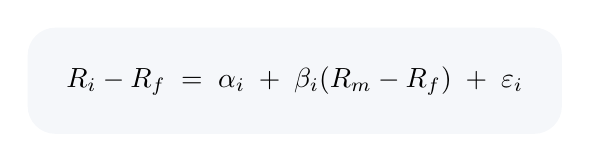
\begin{tikzpicture}
      \node[fill=soft,rounded corners=10pt,
        inner sep=14pt]{%
        $\displaystyle
          R_i - R_f \;=\; \alpha_i
          \;+\; \beta_i\!\left(R_m - R_f\right)
          \;+\; \varepsilon_i
        $};
    \end{tikzpicture}
  \end{center}

  \vspace{0.5cm}
  {\fontsize{13}{18}\selectfont\color{muted}
    \begin{tabular}{@{}r@{\;\;=\;\;}l@{}}
      $R_i - R_f$ & stock excess return\\[3pt]
      $R_m - R_f$ & market excess return\\[3pt]
      $\beta_i$   & sensitivity to the market\\[3pt]
      $\alpha_i$  & abnormal return (skill?)
    \end{tabular}
  }

  \vspace{0.5cm}
  \accentcallout{%
    {\fontsize{14}{18}\selectfont
    If CAPM is right, $\alpha_i = 0$
    for every stock.  Any excess return
    is just \textbf{compensation for risk}.}}

  \swipe
  \vspace{0.3cm}
\end{frame}

% -------------------------------------------------------
%  SLIDE 4 — THE ANOMALY
% -------------------------------------------------------
\begin{frame}[plain,shrink=25]
  \vspace{0.8cm}
  \slidenum{02}
  \hspace{0.2cm}{\large\color{muted}\textbf{CAPM BREAKS DOWN}}

  \vspace{0.4cm}
  {\fontsize{15}{20}\selectfont\color{ink}%
    Two groups of stocks consistently earn
    returns \textbf{too high} for their beta:}

  \vspace{0.5cm}
  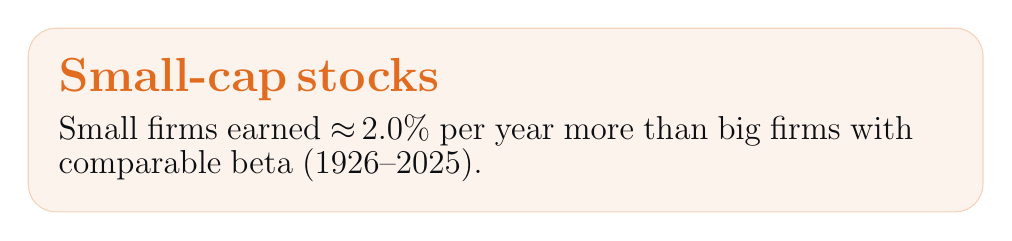
\begin{tikzpicture}
    \node[fill=accentorange!8,draw=accentorange!30,
      rounded corners=10pt,inner sep=11pt,
      text width=\dimexpr\linewidth-22pt\relax]{%
      {\fontsize{16}{20}\selectfont\bfseries
        \color{accentorange}Small-cap stocks}\\[4pt]
      {\fontsize{13}{17}\selectfont\color{ink}%
        Small firms earned $\approx$\,2.0\% per year
        more than big firms with comparable beta
        (1926--2025).}};
  \end{tikzpicture}

  \vspace{0.35cm}
  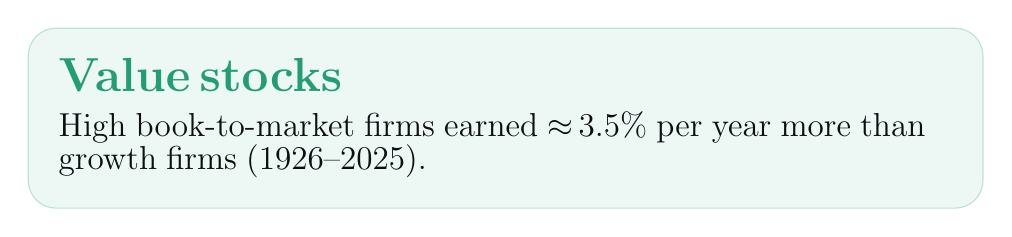
\begin{tikzpicture}
    \node[fill=accentgreen!8,draw=accentgreen!30,
      rounded corners=10pt,inner sep=11pt,
      text width=\dimexpr\linewidth-22pt\relax]{%
      {\fontsize{16}{20}\selectfont\bfseries
        \color{accentgreen}Value stocks}\\[4pt]
      {\fontsize{13}{17}\selectfont\color{ink}%
        High book-to-market firms earned
        $\approx$\,3.5\% per year more than growth
        firms (1926--2025).}};
  \end{tikzpicture}

  \vspace{0.35cm}
  \callout{%
    {\fontsize{13}{17}\selectfont
    These ``anomalies'' persist across countries
    and decades.  CAPM cannot explain them.}\\[4pt]
    {\fontsize{11}{14}\selectfont\color{muted}%
    Data: Kenneth French's Data Library,
    mba.tuck.dartmouth.edu}}

  \swipe
  \vspace{0.2cm}
\end{frame}

% -------------------------------------------------------
%  SLIDE 5 — THE THREE FACTORS
% -------------------------------------------------------
\begin{frame}[plain,shrink=25]
  \vspace{0.8cm}
  \slidenum{03}
  \hspace{0.2cm}{\large\color{muted}\textbf{THREE FACTORS}}

  \vspace{0.4cm}
  {\fontsize{15}{20}\selectfont\color{ink}%
    Fama \& French (1993) add two factors
    to capture the premia CAPM misses:}

  \vspace{0.4cm}
  \begin{center}
    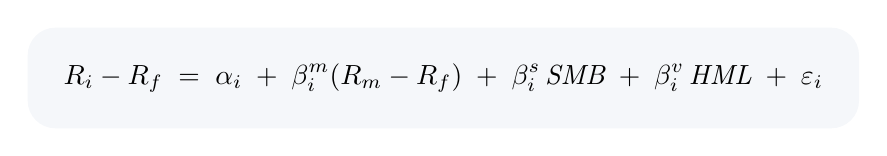
\begin{tikzpicture}
      \node[fill=soft,rounded corners=10pt,
        inner sep=13pt]{%
        $\displaystyle
          R_i - R_f \;=\; \alpha_i
          \;+\; \beta_i^m\!\left(R_m - R_f\right)
          \;+\; \beta_i^s\,\textit{SMB}
          \;+\; \beta_i^v\,\textit{HML}
          \;+\; \varepsilon_i
        $};
    \end{tikzpicture}
  \end{center}

  \vspace{0.4cm}
  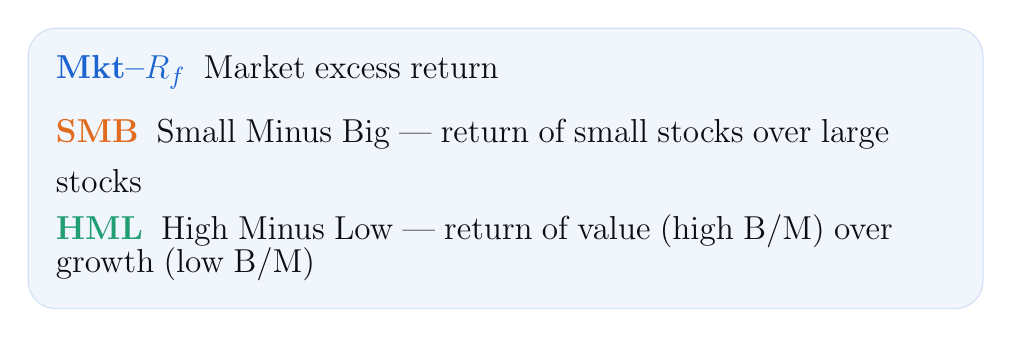
\begin{tikzpicture}
    \node[fill=accent!6,draw=accent!20,
      rounded corners=10pt,inner sep=10pt,
      text width=\dimexpr\linewidth-20pt\relax]{%
      {\fontsize{13}{18}\selectfont\color{ink}
      \textbf{\color{accent}Mkt--$R_f$}\;\;%
        Market excess return\\[5pt]
      \textbf{\color{accentorange}SMB}\;\;%
        Small Minus Big --- return of small
        stocks over large stocks\\[5pt]
      \textbf{\color{accentgreen}HML}\;\;%
        High Minus Low --- return of
        value (high B/M) over growth (low B/M)}};
  \end{tikzpicture}

  \vspace{0.35cm}
  \accentcallout{%
    {\fontsize{14}{18}\selectfont
    If $\alpha_i$ drops to zero under FF3,
    the fund was harvesting
    \textbf{factor premia} --- not generating skill.}}

  \swipe
  \vspace{0.2cm}
\end{frame}

% -------------------------------------------------------
%  SLIDE 6 — FACTOR PREMIA TABLE (real data)
% -------------------------------------------------------
\begin{frame}[plain,shrink=25]
  \vspace{0.8cm}
  \slidenum{04}
  \hspace{0.2cm}{\large\color{muted}%
    \textbf{HISTORICAL FACTOR RETURNS}}

  \vspace{0.3cm}
  {\fontsize{13}{17}\selectfont\color{muted}%
    \hspace{0.2cm}Average annual returns (\%),
    U.S.\ equity, 1926--2025}

  \vspace{0.4cm}
  \begin{center}
    {\fontsize{14}{18}\selectfont
    \begin{tabular}{@{}lcccc@{}}
      \toprule
      \textbf{Factor} & \textbf{Mean} & \textbf{Std Dev}
        & \textbf{Sharpe} & \textbf{$t$-stat}\\
      \midrule
      Mkt--$R_f$ & 8.3 & 20.3 & 0.41 & 4.0\\[3pt]
      SMB        & 2.0 &  11.1 & 0.18 & 1.8\\[3pt]
      HML        & 3.5 &  11.8 & 0.30 & 2.9\\
      \bottomrule
    \end{tabular}}
  \end{center}

  \vspace{0.4cm}
  \callout{%
    {\fontsize{13}{17}\selectfont
    The market premium is the largest and most
    reliable.  The value premium (HML) has been
    historically strong but \textbf{weakened after 2005}.
    The size premium (SMB) is smaller and noisier.}}

  \vspace{0.25cm}
  {\fontsize{10}{13}\selectfont\color{linegray}\centering
    Source: Kenneth French's Data Library.
    Mkt--$R_f$, SMB, HML monthly returns,
    annualised.\par}

  \swipe
  \vspace{0.2cm}
\end{frame}

% -------------------------------------------------------
%  SLIDE 7 — CUMULATIVE FACTOR RETURNS PLOT
% -------------------------------------------------------
\begin{frame}[plain,shrink=25]
  \vspace{0.5cm}
  {\large\color{muted}\bfseries\hspace{0.3cm}%
    GROWTH OF \$1 IN EACH FACTOR}

  \vspace{0.05cm}
  {\fontsize{11}{14}\selectfont\color{linegray}%
    \hspace{0.3cm}Log scale, 1926--2025}

  \vspace{0.1cm}
  \begin{center}
    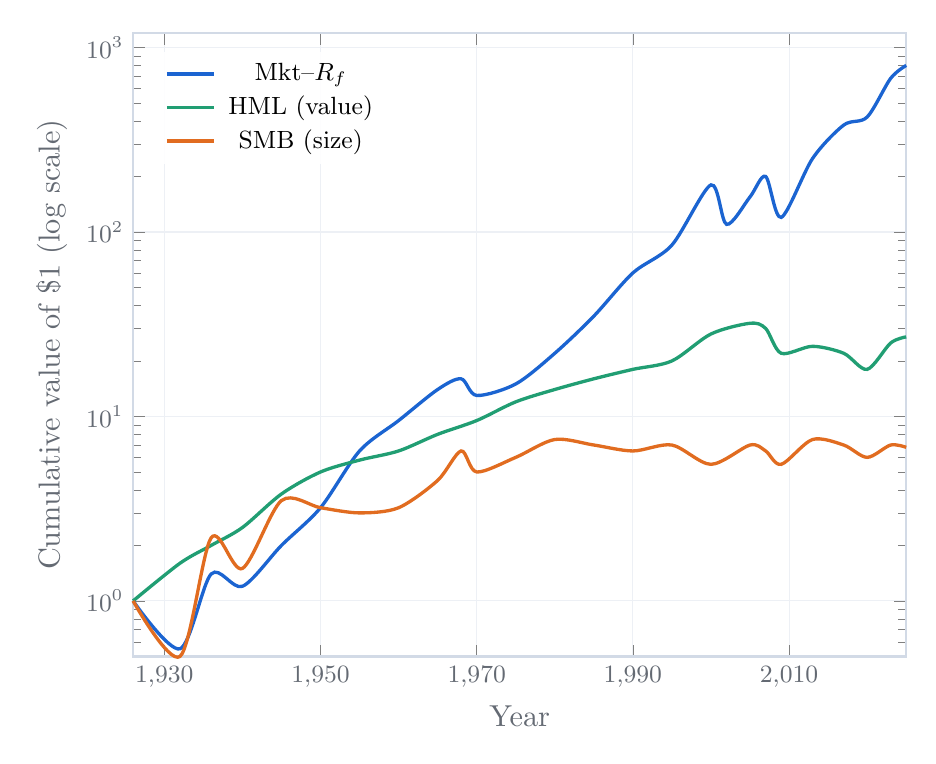
\begin{tikzpicture}
      \begin{axis}[
        width=11.4cm,
        height=9.5cm,
        xlabel={\fontsize{11}{13}\selectfont Year},
        ylabel={\fontsize{11}{13}\selectfont
          Cumulative value of \$1 (log scale)},
        ticklabel style={font=\small,color=muted},
        label style={color=muted},
        axis line style={draw=linegray,thick},
        grid=major,
        grid style={draw=linegray!40},
        xmin=1926,xmax=2025,
        ymode=log,
        ymin=0.5,ymax=1200,
        xtick={1930,1950,1970,1990,2010},
        legend style={font=\small,draw=none,
          fill=white,fill opacity=0.9,text opacity=1,
          at={(0.03,0.97)},anchor=north west},
        clip=false
      ]
        % Market (Mkt-RF): ~8.3% annual → ~$800 by 2025
        \addplot[very thick,accent,smooth]
          coordinates{
            (1926,1)(1932,0.55)(1936,1.4)(1940,1.2)
            (1945,2.0)(1950,3.2)(1955,6.5)(1960,9.5)
            (1965,14)(1968,16)(1970,13)(1975,15)
            (1980,22)(1985,35)(1990,60)(1995,85)
            (2000,180)(2002,110)(2005,155)(2007,200)
            (2009,120)(2013,250)(2017,380)(2020,420)
            (2023,680)(2025,800)
          };
        \addlegendentry{\;Mkt--$R_f$}

        % HML: ~3.5% annual → ~$27 by 2025
        \addplot[very thick,accentgreen,smooth]
          coordinates{
            (1926,1)(1932,1.6)(1936,2.0)(1940,2.5)
            (1945,3.8)(1950,5.0)(1955,5.8)(1960,6.5)
            (1965,8.0)(1970,9.5)(1975,12)(1980,14)
            (1985,16)(1990,18)(1995,20)(2000,28)
            (2005,32)(2007,30)(2009,22)(2013,24)
            (2017,22)(2020,18)(2023,25)(2025,27)
          };
        \addlegendentry{\;HML (value)}

        % SMB: ~2.0% annual → ~$7 by 2025
        \addplot[very thick,accentorange,smooth]
          coordinates{
            (1926,1)(1932,0.5)(1936,2.2)(1940,1.5)
            (1945,3.5)(1950,3.2)(1955,3.0)(1960,3.2)
            (1965,4.5)(1968,6.5)(1970,5.0)(1975,6.0)
            (1980,7.5)(1985,7.0)(1990,6.5)(1995,7.0)
            (2000,5.5)(2005,7.0)(2007,6.5)(2009,5.5)
            (2013,7.5)(2017,7.0)(2020,6.0)(2023,7.0)
            (2025,6.8)
          };
        \addlegendentry{\;SMB (size)}

      \end{axis}
    \end{tikzpicture}
  \end{center}

  \vspace{0.05cm}
  {\fontsize{10}{13}\selectfont\centering\color{linegray}%
    Source: Kenneth French's Data Library.
    Monthly factor returns compounded.\par}

  \swipe
  \vspace{0.15cm}
\end{frame}

% -------------------------------------------------------
%  SLIDE 8 — ALPHA DISAPPEARS
% -------------------------------------------------------
\begin{frame}[plain,shrink=25]
  \vspace{0.8cm}
  \slidenum{05}
  \hspace{0.2cm}{\large\color{muted}%
    \textbf{ALPHA DISAPPEARS}}

  \vspace{0.4cm}
  {\fontsize{14}{19}\selectfont\color{ink}%
    A fund returns 12\%/year when the market
    returns 8\%.  Under CAPM that is 4\% alpha.
    But the fund loads on small and value stocks:}

  \vspace{0.4cm}
  \begin{center}
    {\fontsize{13}{17}\selectfont
    \begin{tabular}{@{}lcc@{}}
      \toprule
      & \textbf{CAPM} & \textbf{FF3}\\
      \midrule
      $\alpha$ (annual)
        & \textbf{\color{accentgreen}+4.0\%}
        & \textbf{\color{muted}+0.3\%}\\[4pt]
      $\beta^{m}$ & 1.05 & 0.98\\[4pt]
      $\beta^{s}$ (SMB)
        & --- & \textbf{\color{accentorange}0.65}\\[4pt]
      $\beta^{v}$ (HML)
        & --- & \textbf{\color{accentgreen}0.72}\\[4pt]
      $R^2$ & 0.78 & 0.93\\
      \bottomrule
    \end{tabular}}
  \end{center}

  \vspace{0.4cm}
  \accentcallout{%
    {\fontsize{14}{18}\selectfont
    The ``alpha'' was just a \textbf{size premium}
    ($\beta^s\!\times\!$SMB) plus a \textbf{value premium}
    ($\beta^v\!\times\!$HML).  No skill required.}}

  \swipe
  \vspace{0.2cm}
\end{frame}

% -------------------------------------------------------
%  SLIDE 9 — VALUE PREMIUM BY DECADE
% -------------------------------------------------------
\begin{frame}[plain,shrink=25]
  \vspace{0.5cm}
  {\large\color{muted}\bfseries\hspace{0.3cm}%
    VALUE PREMIUM BY DECADE}

  \vspace{0.05cm}
  {\fontsize{11}{14}\selectfont\color{linegray}%
    \hspace{0.3cm}Average annual HML return (\%)}

  \vspace{0.15cm}
  \begin{center}
    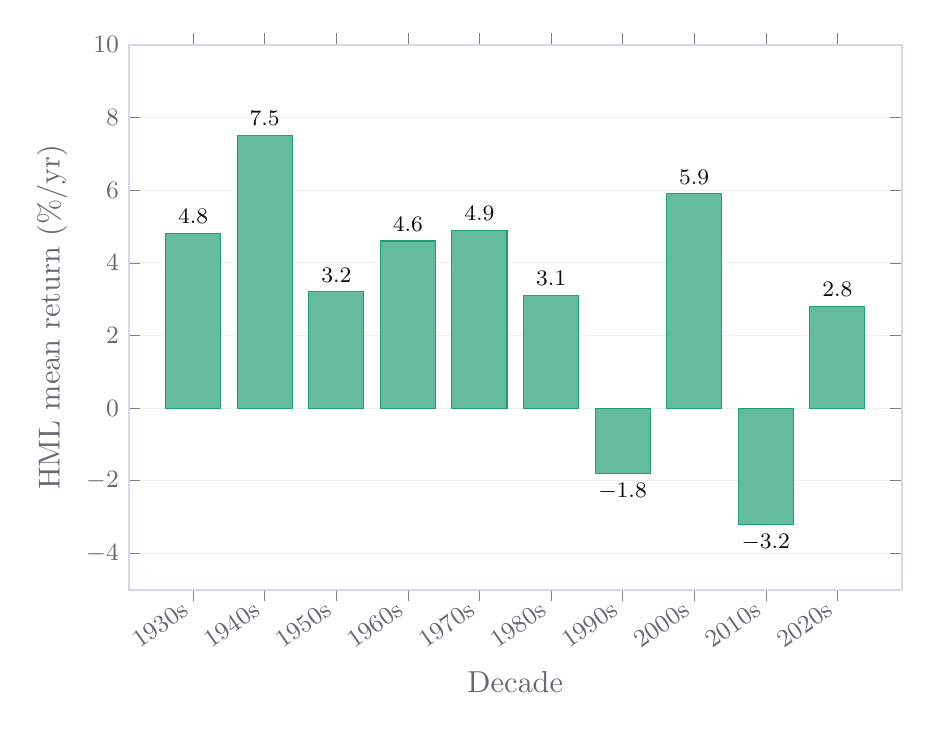
\begin{tikzpicture}
      \begin{axis}[
        width=11.4cm,
        height=8.5cm,
        ybar,
        bar width=0.7cm,
        xlabel={\fontsize{11}{13}\selectfont Decade},
        ylabel={\fontsize{11}{13}\selectfont
          HML mean return (\%/yr)},
        ticklabel style={font=\small,color=muted},
        label style={color=muted},
        axis line style={draw=linegray,thick},
        ymajorgrids=true,
        grid style={draw=linegray!40},
        ymin=-5,ymax=10,
        xtick=data,
        xticklabels={1930s,1940s,1950s,1960s,
          1970s,1980s,1990s,2000s,2010s,2020s},
        xticklabel style={rotate=35,anchor=east,
          font=\small},
        nodes near coords,
        every node near coord/.append style={
          font=\footnotesize\bfseries,color=ink},
        clip=false
      ]
        \addplot[fill=accentgreen!70,draw=accentgreen]
          coordinates{
            (1,4.8)(2,7.5)(3,3.2)(4,4.6)
            (5,4.9)(6,3.1)(7,-1.8)(8,5.9)(9,-3.2)
            (10,2.8)
          };
      \end{axis}
    \end{tikzpicture}
  \end{center}

  \vspace{0.1cm}
  \callout{%
    {\fontsize{13}{17}\selectfont
    The value premium was strong for seven decades,
    then \textbf{turned negative} in the 1990s
    and 2010s.  It staged a partial comeback
    in the 2020s --- but ``is value dead?''
    remains one of the biggest debates in finance.}}

  \swipe
  \vspace{0.15cm}
\end{frame}

% -------------------------------------------------------
%  SLIDE 10 — FIVE FACTORS
% -------------------------------------------------------
\begin{frame}[plain,shrink=25]
  \vspace{0.8cm}
  \slidenum{06}
  \hspace{0.2cm}{\large\color{muted}%
    \textbf{THE FIVE-FACTOR MODEL}}

  \vspace{0.4cm}
  {\fontsize{14}{19}\selectfont\color{ink}%
    Fama \& French (2015) add two more factors
    to capture profitability and investment
    patterns:}

  \vspace{0.35cm}
  \begin{center}
    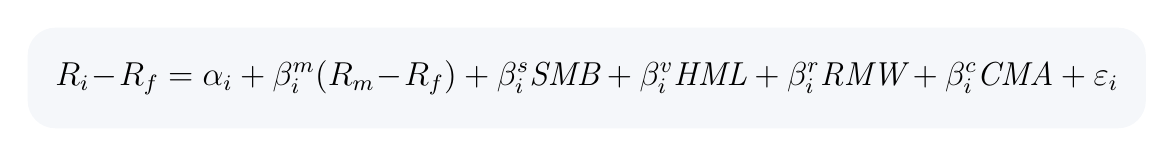
\begin{tikzpicture}
      \node[fill=soft,rounded corners=10pt,
        inner xsep=10pt,inner ysep=12pt]{%
        \fontsize{12}{16}\selectfont$\displaystyle
          R_i \!-\! R_f = \alpha_i
          + \beta_i^m(R_m \!-\! R_f)
          + \beta_i^s \textit{SMB}
          + \beta_i^v \textit{HML}
          + \beta_i^r \textit{RMW}
          + \beta_i^c \textit{CMA}
          + \varepsilon_i
        $};
    \end{tikzpicture}
  \end{center}

  \vspace{0.35cm}
  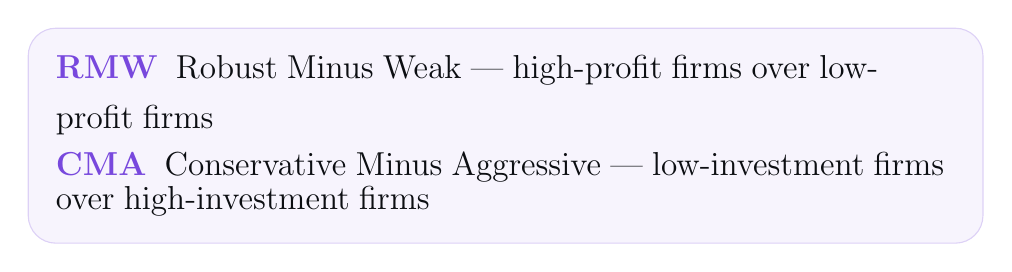
\begin{tikzpicture}
    \node[fill=accentpurple!6,draw=accentpurple!25,
      rounded corners=10pt,inner sep=10pt,
      text width=\dimexpr\linewidth-20pt\relax]{%
      {\fontsize{13}{18}\selectfont\color{ink}
      \textbf{\color{accentpurple}RMW}\;\;%
        Robust Minus Weak ---
        high-profit firms over low-profit firms\\[5pt]
      \textbf{\color{accentpurple}CMA}\;\;%
        Conservative Minus Aggressive ---
        low-investment firms over
        high-investment firms}};
  \end{tikzpicture}

  \vspace{0.3cm}
  \callout{%
    {\fontsize{13}{17}\selectfont
    RMW $\approx$ 3.2\%/yr,\;\;
    CMA $\approx$ 3.0\%/yr\;\;(1963--2025).\\[3pt]
    Adding these two factors makes HML
    largely redundant --- value is partly
    explained by profitability and investment.}}

  \swipe
  \vspace{0.2cm}
\end{frame}

% -------------------------------------------------------
%  SLIDE 11 — HOW FACTORS ARE CONSTRUCTED
% -------------------------------------------------------
\begin{frame}[plain,shrink=25]
  \vspace{0.7cm}
  \slidenum{07}
  \hspace{0.2cm}{\large\color{muted}%
    \textbf{HOW SMB \& HML ARE BUILT}}

  \vspace{0.4cm}
  \begin{center}
    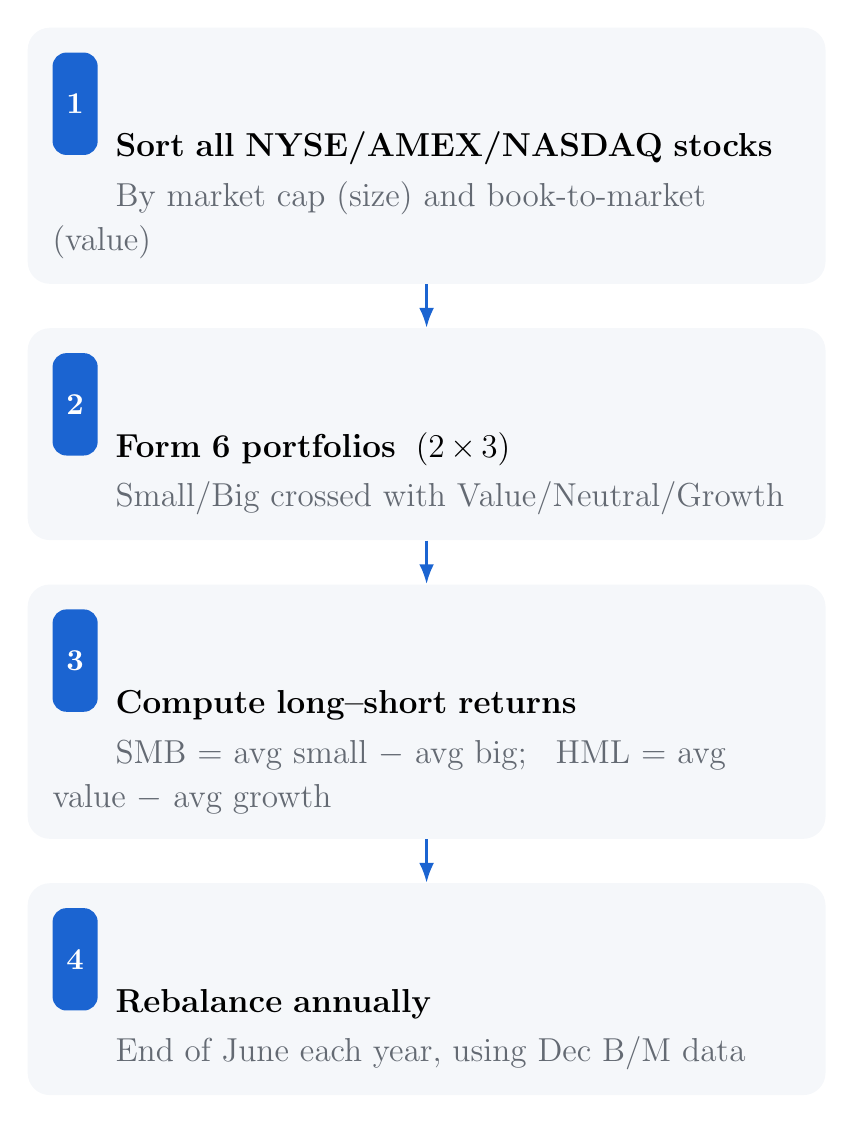
\begin{tikzpicture}[
      node distance=0.55cm,
      box/.style={fill=soft,rounded corners=8pt,
        text width=9.5cm,minimum height=1.3cm,
        align=left,inner sep=9pt,
        font=\fontsize{12}{16}\selectfont},
      numstyle/.style={fill=accent,text=white,
        rounded corners=5pt,
        font=\fontsize{11}{13}\selectfont\bfseries,
        inner xsep=5pt,inner ysep=2pt},
      arr/.style={-{Latex[length=2.5mm]},thick,accent}
    ]
      \node[box](s1){%
        \makebox[0pt][l]{\raisebox{0.02cm}{%
          \tikz\node[numstyle]{1};}}%
        \hspace{0.8cm}\textbf{Sort all NYSE/AMEX/NASDAQ
          stocks}\\[2pt]
        \hspace{0.8cm}\color{muted}%
          By market cap (size) and book-to-market (value)};

      \node[box,below=of s1](s2){%
        \makebox[0pt][l]{\raisebox{0.02cm}{%
          \tikz\node[numstyle]{2};}}%
        \hspace{0.8cm}\textbf{Form 6 portfolios}
          \;(2\,$\times$\,3)\\[2pt]
        \hspace{0.8cm}\color{muted}%
          Small/Big crossed with Value/Neutral/Growth};

      \node[box,below=of s2](s3){%
        \makebox[0pt][l]{\raisebox{0.02cm}{%
          \tikz\node[numstyle]{3};}}%
        \hspace{0.8cm}\textbf{Compute long--short returns}\\[2pt]
        \hspace{0.8cm}\color{muted}%
          SMB = avg small $-$ avg big;\;\;
          HML = avg value $-$ avg growth};

      \node[box,below=of s3](s4){%
        \makebox[0pt][l]{\raisebox{0.02cm}{%
          \tikz\node[numstyle]{4};}}%
        \hspace{0.8cm}\textbf{Rebalance annually}\\[2pt]
        \hspace{0.8cm}\color{muted}%
          End of June each year, using Dec B/M data};

      \draw[arr](s1)--(s2);
      \draw[arr](s2)--(s3);
      \draw[arr](s3)--(s4);
    \end{tikzpicture}
  \end{center}

  \vspace{0.2cm}
  {\fontsize{10}{13}\selectfont\centering\color{linegray}%
    Source: Fama \& French (1993),
    \textit{J.\ Financial Economics}, 33(1), 3--56.\par}

  \swipe
  \vspace{0.2cm}
\end{frame}

% -------------------------------------------------------
%  SLIDE 12 — PRACTICAL USES
% -------------------------------------------------------
\begin{frame}[plain,shrink=25]
  \vspace{0.7cm}
  \slidenum{08}
  \hspace{0.2cm}{\large\color{muted}%
    \textbf{WHY THIS MATTERS}}

  \vspace{0.4cm}
  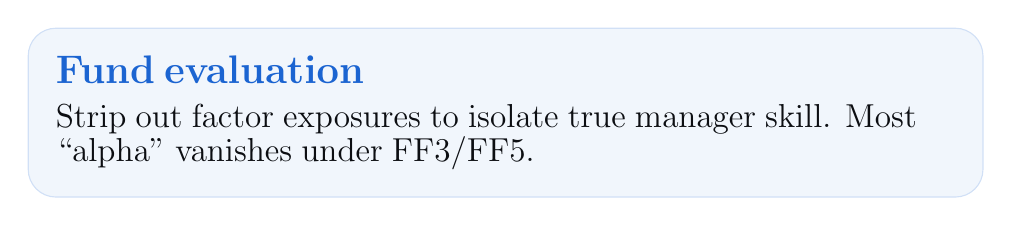
\begin{tikzpicture}
    \node[fill=accent!6,draw=accent!20,
      rounded corners=10pt,inner sep=10pt,
      text width=\dimexpr\linewidth-20pt\relax]{%
      {\fontsize{15}{19}\selectfont\bfseries
        \color{accent}Fund evaluation}\\[4pt]
      {\fontsize{13}{17}\selectfont\color{ink}%
        Strip out factor exposures to isolate
        true manager skill.  Most ``alpha''
        vanishes under FF3/FF5.}};
  \end{tikzpicture}

  \vspace{0.3cm}
  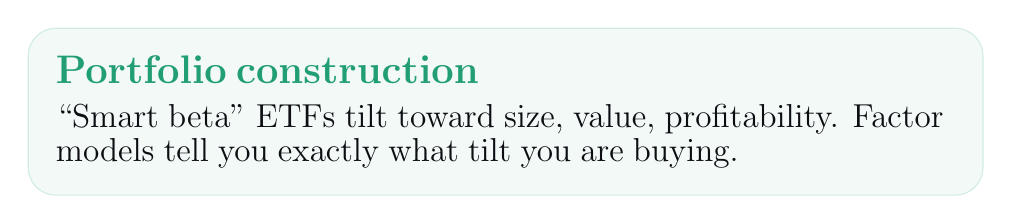
\begin{tikzpicture}
    \node[fill=accentgreen!6,draw=accentgreen!20,
      rounded corners=10pt,inner sep=10pt,
      text width=\dimexpr\linewidth-20pt\relax]{%
      {\fontsize{15}{19}\selectfont\bfseries
        \color{accentgreen}Portfolio construction}\\[4pt]
      {\fontsize{13}{17}\selectfont\color{ink}%
        ``Smart beta'' ETFs tilt toward size,
        value, profitability.  Factor models
        tell you exactly what tilt you are buying.}};
  \end{tikzpicture}

  \vspace{0.3cm}
  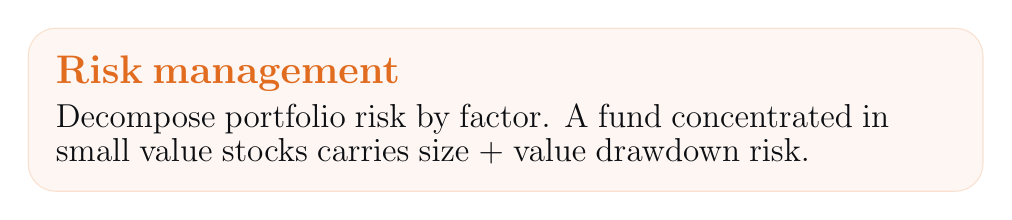
\begin{tikzpicture}
    \node[fill=accentorange!6,draw=accentorange!20,
      rounded corners=10pt,inner sep=10pt,
      text width=\dimexpr\linewidth-20pt\relax]{%
      {\fontsize{15}{19}\selectfont\bfseries
        \color{accentorange}Risk management}\\[4pt]
      {\fontsize{13}{17}\selectfont\color{ink}%
        Decompose portfolio risk by factor.
        A fund concentrated in small value
        stocks carries size + value drawdown risk.}};
  \end{tikzpicture}

  \swipe
  \vspace{0.2cm}
\end{frame}

% -------------------------------------------------------
%  SLIDE 13 — FACTOR ZOO & CRITICISM
% -------------------------------------------------------
\begin{frame}[plain,shrink=25]
  \vspace{0.7cm}
  \slidenum{09}
  \hspace{0.2cm}{\large\color{muted}%
    \textbf{THE FACTOR ZOO}}

  \vspace{0.4cm}
  {\fontsize{15}{20}\selectfont\color{ink}%
    Researchers have published \textbf{400+}
    factors.  Most are spurious.}

  \vspace{0.4cm}
  \callout{%
    {\fontsize{13}{17}\selectfont
    Harvey, Liu \& Zhu (2016) show that the
    standard $t > 2$ threshold produces
    massive false discoveries when applied
    across hundreds of tested factors.  They
    recommend $t > 3$ for new factors.}}

  \vspace{0.35cm}
  {\fontsize{14}{19}\selectfont\color{ink}%
    The Fama--French factors survive scrutiny
    because they are:}

  \vspace{0.25cm}
  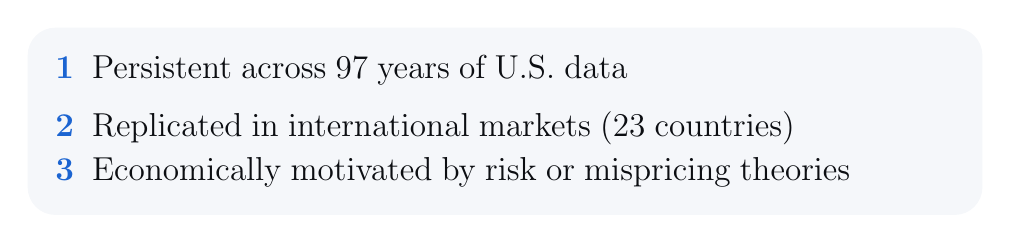
\begin{tikzpicture}
    \node[fill=soft,rounded corners=10pt,inner sep=10pt,
      text width=\dimexpr\linewidth-20pt\relax]{%
      {\fontsize{13}{17}\selectfont\color{ink}
      \textbf{\color{accent}1}\;\;Persistent across
        97 years of U.S.\ data\\[4pt]
      \textbf{\color{accent}2}\;\;Replicated in
        international markets (23 countries)\\[4pt]
      \textbf{\color{accent}3}\;\;Economically motivated
        by risk or mispricing theories}};
  \end{tikzpicture}

  \swipe
  \vspace{0.2cm}
\end{frame}

% -------------------------------------------------------
%  SLIDE 14 — KEY REFERENCES
% -------------------------------------------------------
\begin{frame}[plain,shrink=25]
  \vspace{0.7cm}
  \slidenum{10}
  \hspace{0.2cm}{\large\color{muted}\textbf{GO DEEPER}}

  \vspace{0.4cm}
  {\fontsize{12}{17}\selectfont\color{ink}

  \textbf{\color{accent}Original papers}\\[5pt]
  Fama, E.\ \& French, K.\ (1993).\ Common risk factors
  in the returns on stocks and bonds.\
  \textit{J.\ Financial Economics}, 33(1), 3--56.\\[4pt]
  Fama, E.\ \& French, K.\ (2015).\ A five-factor
  asset pricing model.\
  \textit{J.\ Financial Economics}, 116(1), 1--22.

  \vspace{0.3cm}
  \textbf{\color{accent}On the factor zoo}\\[5pt]
  Harvey, C., Liu, Y.\ \& Zhu, H.\ (2016).\
  \ldots and the cross-section of expected returns.\
  \textit{Review of Financial Studies}, 29(1), 5--68.

  \vspace{0.3cm}
  \textbf{\color{accent}Data}\\[5pt]
  Kenneth French's Data Library\\
  {\color{muted}\texttt{mba.tuck.dartmouth.edu/pages/\\
  faculty/ken.french/data\_library.html}}
  }

  \swipe
  \vspace{0.2cm}
\end{frame}

% -------------------------------------------------------
%  SLIDE 15 — TAKEAWAY
% -------------------------------------------------------
\begin{frame}[plain,shrink=25]
  \vfill
  \begin{center}
    {\fontsize{14}{18}\selectfont\color{accent}\bfseries%
      TAKEAWAY}\\[0.6cm]
    {\fontsize{24}{30}\selectfont\bfseries\color{ink}%
      Your alpha is someone\\[0.15cm]
      else's beta.}\\[0.8cm]
    {\fontsize{15}{20}\selectfont\color{muted}%
      Before calling a manager skilled,\\[0.1cm]
      check whether the returns are just\\[0.1cm]
      compensation for exposure to\\[0.1cm]
      \textbf{\color{accentorange}size},
      \textbf{\color{accentgreen}value},
      \textbf{\color{accentpurple}profitability},
      and \textbf{\color{accent}investment}.}\\[0.7cm]
    {\fontsize{14}{18}\selectfont\color{ink}%
      Fama--French gave us the tools\\[0.1cm]
      to decompose returns and separate\\[0.1cm]
      \textbf{risk premia from genuine skill}.}
  \end{center}
  \vfill
  \swipe
  \vspace{0.3cm}
\end{frame}

% -------------------------------------------------------
%  SLIDE 16 — THANK YOU
% -------------------------------------------------------
\setbeamertemplate{footline}{}
\begin{frame}[plain,shrink=25]
  \vspace{2.5cm}
  \begin{center}
    {\fontsize{28}{32}\selectfont\bfseries\color{ink}%
      Thank You}\\[0.8cm]
    {\fontsize{16}{20}\selectfont\color{ink}%
      Muiz Olasupo}\\[0.3cm]
    {\fontsize{13}{17}\selectfont\color{muted}%
      Quantitative Finance}\\[0.15cm]
    {\fontsize{13}{17}\selectfont\color{muted}%
      April 2026}
  \end{center}
  \vfill
\end{frame}

\end{document}
